% Source-coordinate reconstruction. Edit named defaults or copy this entire composition.
\studiodeclarefield{graphic-1}{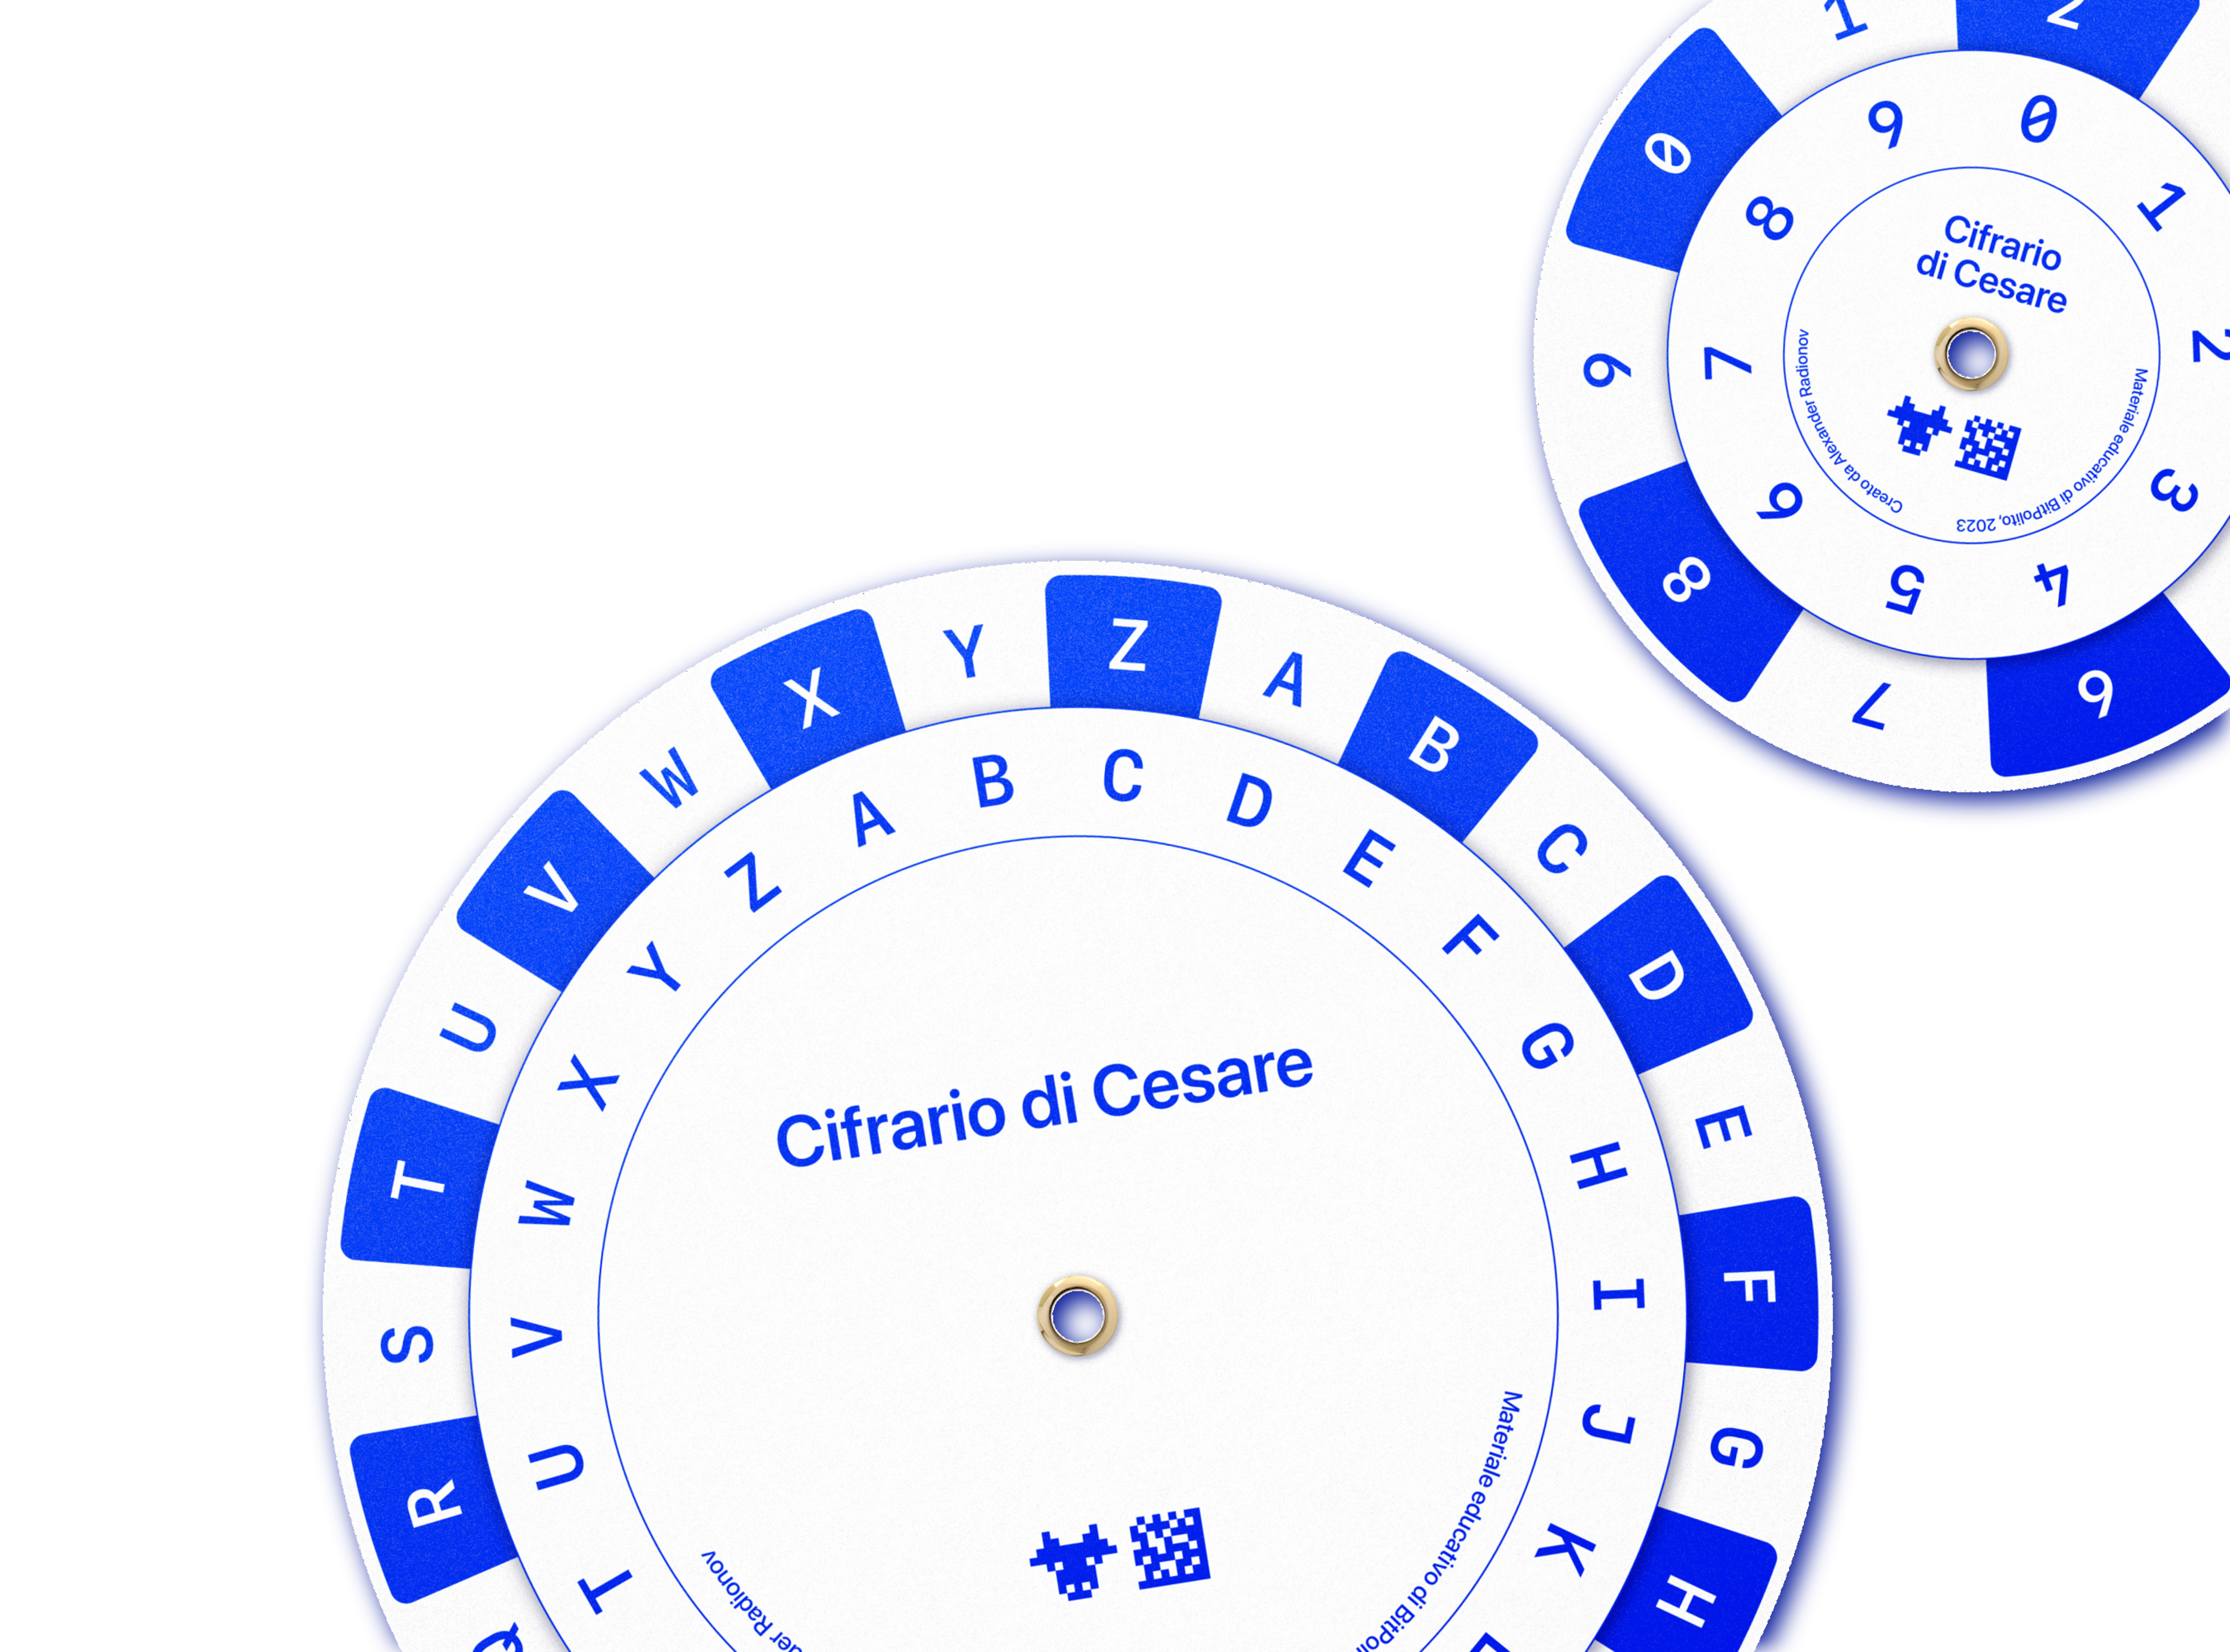
\includegraphics[width=2700\studiounit]{images/studio/collection/figma-0508-part-01.pdf}}
\studiodeclarefield{title}{Caesar cipher}
\studiodeclarefield{item-2-1}{One of the earliest examples}
\studiodeclarefield{item-2-2}{of cryptography.}
\studiodeclarefield{item-2-3}{To communicate securely with his}
\studiodeclarefield{item-2-4}{generals, Julius Caesar encrypted}
\studiodeclarefield{item-2-5}{his messages so that only}
\studiodeclarefield{item-2-6}{authorized people could}
\studiodeclarefield{item-2-7}{understand their content.}
\studiodeclarefield{text-3}{Roman era}
\studioapplyfields
\studiomeasuredcanvas{3556}{2000}{cipher-wheel}{studio-paper}{
\studiomeasuredtext{title}{304.57}{260.047}{980.676}{152.571}{116.641}{135.304}{\color{bitpolito}\bfseries}{\studiofield{title}}
\studiomeasuredtext{item-2-1}{304.546}{441.209}{1111.46}{98.9227}{65.7613}{76.2831}{\color{bitpolito}}{\studiofield{item-2-1}}
\studiomeasuredtext{item-2-2}{302.051}{525.961}{1377.63}{99.4153}{66.7187}{77.3937}{\color{bitpolito}}{\studiofield{item-2-2}}
\studiomeasuredtext{item-2-3}{304.546}{693.995}{1178.41}{78.1196}{49.812}{57.7819}{\color{bitpolito}}{\studiofield{item-2-3}}
\studiomeasuredtext{item-2-4}{302.085}{777.858}{1101.69}{98.9925}{65.7627}{76.2847}{\color{bitpolito}}{\studiofield{item-2-4}}
\studiomeasuredtext{item-2-5}{302.085}{861.995}{1081.93}{98.8547}{65.7613}{76.2831}{\color{bitpolito}}{\studiofield{item-2-5}}
\studiomeasuredtext{item-2-6}{303.623}{945.995}{954.636}{95.7277}{61.3867}{71.2085}{\color{bitpolito}}{\studiofield{item-2-6}}
\studiomeasuredtext{item-2-7}{302.051}{1030}{870.409}{97.6}{64.8}{75.168}{\color{bitpolito}}{\studiofield{item-2-7}}
\studiographfield{graphic-1}{856}{0}{2700}{2000}{}{}
\studiomeasuredtext{text-3}{303.906}{1703.7}{377.233}{100.951}{77.6533}{90.0779}{\color{bitpolito}}{\studiofield{text-3}}
}
